\section{Introduction to Modern Cosmology}

The quest to understand the natural world and how we are placed in it has existed for many centuries. It has influenced many religious, cultural and scientific 
ideas throughout time and their evolutions has led us to how we see our Universe today.
Physical cosmology (hereafter simply cosmology) is the study of the nature of our Universe through observations in order to understand its origins, dynamics and components. 
We consider the beginning of modern cosmology was about a century ago with the discovery of the expansion of the Universe initially predicted by Lemaître in 1927 (\cite{Lemaitre_1927},  \cite{Lemaitre_1931})
and observed by Hubble in 1929 (\cite{Hubble_1929}). The current cosmological model named $\Lambda$CDM ($\Lambda$ Cold Dark Matter) best describes our Universe's 
history, dynamics and components. In this section I will detail the necessary tools that allow us to describe the large scale Universe 
as we know it today. \\

\subsection{General Relativity}

According to modern belief and understanding, the Universe contains four fundamental forces dominating at different scales: at large scales, that force is gravity.
The basis of our understanding of modern cosmology is centered around Einstein's gravitational theory: General Relativity (GR) (\cite{Einstein_1916}), the most tested theory of
gravity to date. GR's views on the nature of gravity differs a lot from the classical Newtonian view. In GR, massive objects do not directly exert a force on other massive objects, but instead 
cause distortions in spacetime. The theory was established after the success of the theory of Special Relativity, also theorized by Einstein in 1905, where the speed of 
light was postulated to be constant in all observation frames and supported by observations.\\

Understanding the mathematical foundation of GR requires a couple of fundamental notions. GR treats coordinate transformations in a 4-dimensional space (spacetime) $(t, x, y, z)$ 
using diffeomorphisms. The formalism will be described using tensorial notations and the Einstein summing convention will also be assumed. We invite the reader to 
familiarise themselves with these notions as well as an understanding of classical field theory. We will also not be going into a lot details 
regarding some mathematical and geometrical notions (like geodesics, covectors, covariant derivatives, etc..) 
and physical concepts found in the Einstein equations such as the Riemann tensor $R^{\mu}_{\nu \kappa \lambda}$, 
Ricci tensor $R_{\mu \nu}$, the Ricci scalar $R$, and Christoffel symbols $\Gamma ^{\mu}_{\nu \lambda}$. If you are interested in learning more on those concepts we 
recommend David Tong's lectures on General Relativity \footnote{\url{https://www.damtp.cam.ac.uk/user/tong/gr.html}}. \\

\noindent \textbf{\underline{Equivalence principle}} \\

Einstein's equivalence principle builds up upon previous results obtained in Newtonian physics. The principle states that the gravitational mass $m_g$ defined due to 
gravitational interactions is equal to the inertial mass $m_i$ which governs the response of an object to an applied force. This previously lead to the idea that free falling objects have 
the same acceleration regardless of their masses. Einstein's principle extends this idea to accelerated frames and not just inertial frames. This principle has been heavily tested 
on Earth and in the Solar System and is yet to be invalidated (REFS). \\


\noindent \textbf{\underline{Einstein equations}} \\

In order to define the equations of motions of any object in GR, the first thing that must be defined is a metric. Physically, a metric is an infinitesimal "separation" that is 
conserved. In classical physics, the length between two points $\Delta L$ would be identical for two observers even if both are moving. In GR this is no longer true and only a 
combination of a spatial separation and a temporal one becomes invariant. If we write down the spacetime displacement as $dx^{\mu}$ with $\mu$ and index taking the values $0$ 
if it is a time displacement and ${1, 2, 3}$ if it is spatial displacement along the $x, y, z$, we can define the invariant displacement $ds^2$ as :
\begin{equation}
    ds^2 = g_{\mu \nu} dx^{\mu} dx^{\nu}
\end{equation}
where $g_{\mu \nu}$ is the metric that can depend on the coordinates $x^{\mu}$. Essentially, the metric expresses the distance between two events in spacetime. An example of a 
metric is the Minkowski metric used to describe events in special relativity and is written as:
\begin{equation}
    \eta_{\mu \nu} =
    \begin{pmatrix}
        +1 & 0 & 0 & 0 \\
        0 & -1 & 0 & 0 \\
        0 & 0 & -1 & 0 \\
        0 & 0 & 0 & -1
    \end{pmatrix}
\end{equation}

Since in GR spacetime can go through a series of curvatures, we do not expect that an object exhibiting no forces to move in a straight line. What we see instead is that 
they follow \textit{geodesics}. One can think of geodesics as the straightest possible path in a curved space. 
The geodesic equation, which corresponds to the equation of motion for a point-like object, is written as:

\begin{equation}
    \frac{d^2 x^{\mu}}{d\lambda^2} + \Gamma^{\mu}_{\alpha \beta} 
    \frac{dx^{\alpha}}{d\lambda} \frac{dx^{\beta}}{d\lambda} = 0
\end{equation}
where $\Gamma^{\mu}_{\alpha \beta}$ are the Christoffel symbols and $\lambda$ is the evolution parameter which increases along the particle's path. 
One can derive the geodesic equation by applying the equivalence principle on a freely falling particle
that does not accelerate (such that $\frac{d^2 x^{\mu}}{d\lambda^2} = 0$). \\

The Einstein field equations (\cite{Einstein_1916}) close the theory by relating the geometry of spacetime, encoded in the metric, to the distribution of matter 
and energy within it. In this framework, gravity is not a force but a manifestation of spacetime curvature, and the motion of particles follows the geodesics of that 
curved geometry. We note $G_{\mu \nu}$ the Einstein tensor describing the geometry and $ T_{\mu \nu} $ the energy-momentum tensor describing the energy content, we get the 
following Einstein equations: 
\begin{equation}
    \boxed{G_{\mu \nu} = R_{\mu \nu} - \frac{1}{2}g_{\mu \nu}R = \frac{8\pi G}{c^4}T_{\mu \nu}}
\end{equation}
where $R_{\mu \nu}$ is the Ricci tensor, $R$ the Ricci scalar, $G$ Newton's gravitational constant and $c$ the speed of light. It is important to note that 
for a symmetric metric, this represents a set of 10 equations where the coefficients of $g_{\mu \nu}$ are unknowns.\\

We can always rewrite the energy momentum tensor as $T_{\mu \nu} = T'_{\mu \nu} - \Lambda g_{\mu \nu}$ where 
$\Lambda$ is a constant that can take any value, even 0. The Einstein equations would be:
\begin{equation}
    R_{\mu \nu} - \frac{1}{2}g_{\mu \nu}R  + \Lambda g_{\mu \nu} = \frac{8\pi G}{c^4}T'_{\mu \nu}
    \label{eqn:einstein_lambda}
\end{equation} 
Physically however, this new expression can lead to different interpretations of the nature behind the accelerated expanding Universe (see Section \ref{sec:expanding_universe}). \\

The Einstein equations could also be determined by varying the Einstein-Hilbert action which is:
\begin{equation}
    S_{EH} = \frac{c^4}{16 \pi G}\int d^4x \sqrt{-g}(R-2\Lambda) + \int d^4x \sqrt{-g} \mathcal{L}_m
\end{equation}
\begin{equation}
    \frac{\delta S_{EH}}{\delta g_{\mu \nu}} = 0
\end{equation}
where $g$ is the determinant of the metric and $\mathcal{L}_m$ is the Lagrangian density of a field that we include in our theory (such as matter, radiation ...).
This is a mathematically rigorous approach to deriving the field equations and it is commonly used when exploring modified theories of gravity (see Section \ref{sec:modified_gravity}).\\

\subsection{The Expanding, Homogeneous Universe} 

\noindent \textbf{\underline{Cosmological principle}} \\

A key principle in modern cosmology is the cosmological principle, stating that the Universe on large scales is homogeneous and isotropic. This is understood in the sense that 
the Universe does not possess a privileged center and that the structures in it remain identical regardless of the direction of observation. Observations from the SDSS 
(Sloan Digital Sky Survey \cite{Sarkar_2009}) and DESI (Dark Energy Spectroscopic Instrument \cite{Adame_2025}) have shown strong evidence for homogeneity in the Universe at 
large scales. We represent this in detail with large scale dark matter simulations such as the Uchuu simulation \cite{Ishiyama_2021} seen in Figure \ref{fig:uchuu_sky}. 
We can see that on large scales the matter distribution is homogeneous. 
CMB measurements from the Planck collaboration (\cite{Planck18_CMB}) have shown strong evidence for isotropy as shown in Figure \ref{fig:cmb}.\\


\begin{figure}[ht]
    \centering
    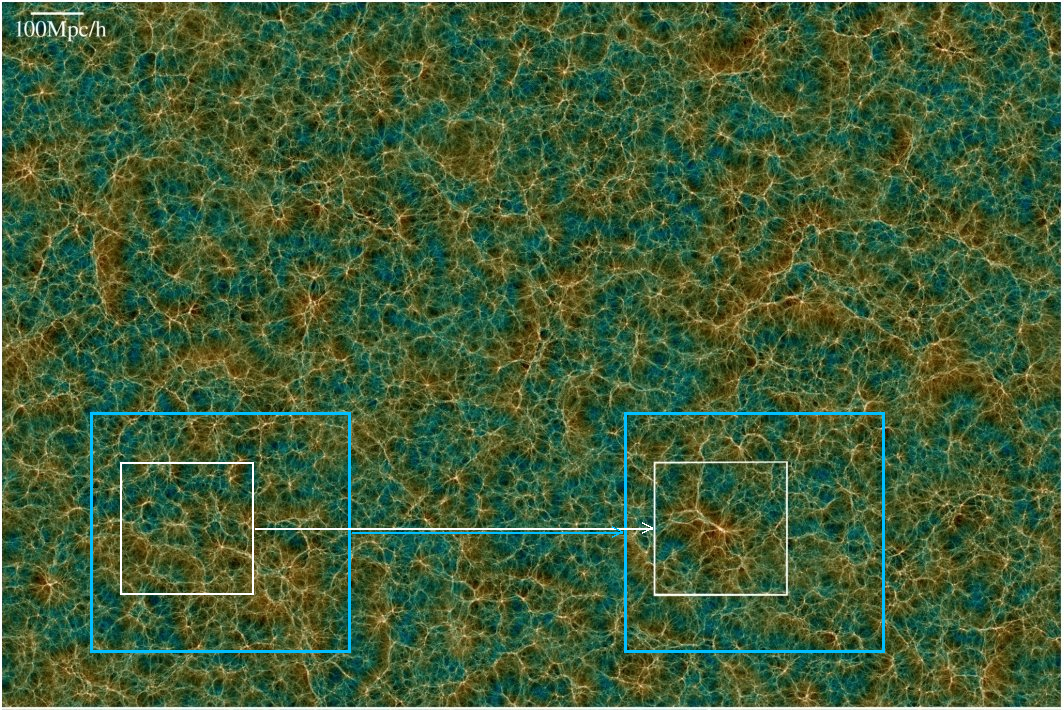
\includegraphics[width=1.0\textwidth]{MainLayout/Introduction_chapter/figures/uchuu_big_box_2.png}
    \caption{Uchuu dark matter simulation of a box $2000 \, \text{Mpc}.h^{-1}$ $\times$ $1333 \, \text{Mpc}.h^{-1}$ with a thickness of $25 \, \text{Mpc}.h^{-1}$. The blue boxes highlight the homogeneity at large scales while the white boxes highlight the inhomogeneity at some scales due to structure formation. Adapted from \cite{Ishiyama_2021}.}
    \label{fig:uchuu_sky}
\end{figure}

\begin{figure}[ht]
    \centering
    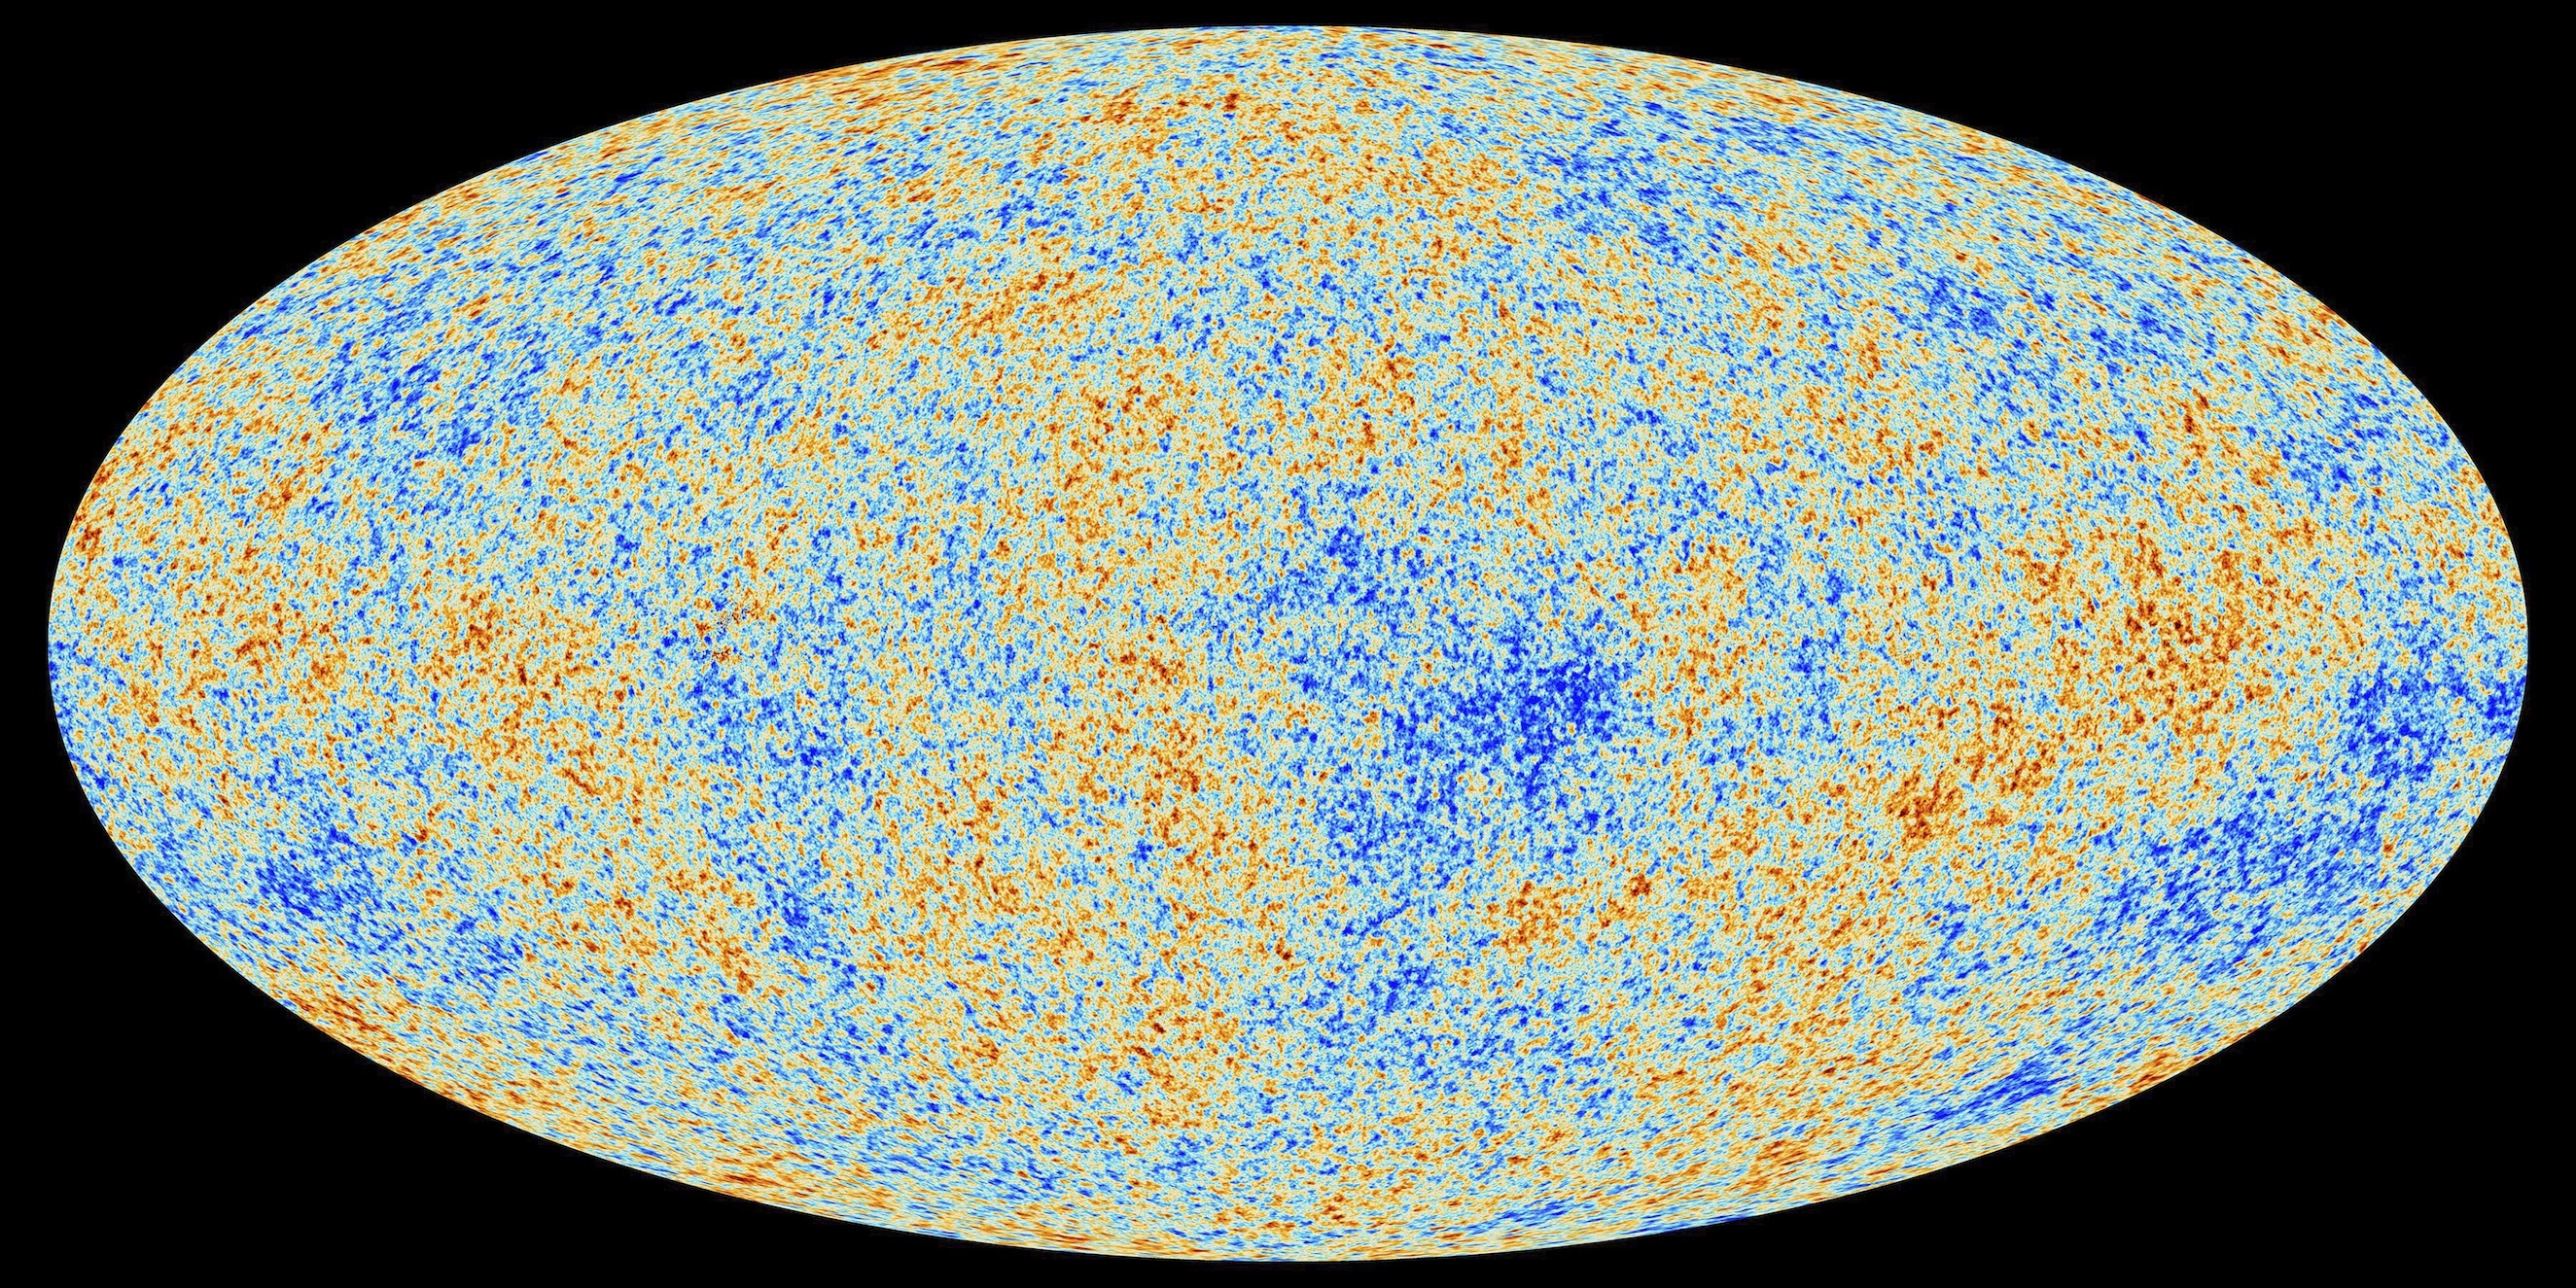
\includegraphics[width=1.0\textwidth]{MainLayout/Introduction_chapter/figures/Cosmic_Microwave_Background_(CMB).jpeg}
    \caption{CMB map provided by ESA and the Planck Collaboration.}
    \label{fig:cmb}
\end{figure}

\noindent \textbf{\underline{Expanding Universe and Hubble relation}} \\

Following the publication of GR, discoveries from \cite{Lemaitre_1927}'s work on the Einstein field equations showed that the proper velocity of a celestial object
was proportional to its distance. Two years later, \cite{Hubble_1929} showed that the radial velocities of 32 nearby galaxies increase with their 
distances indicating an expanding Universe, which is shown in Figure \ref{fig:hubble_og}. The Hubble-Lemaître relation is established as :
\begin{equation}
    v = H_0 d
\end{equation}
where $v$ is the velocity, $d$ the distance of the object and $H_0$ the Hubble constant. Initially, $H_0$ was measured to be around $500 \, \text{km}s^{-1}.\text{Mpc}^{-1}$, 
today more precise measurements show that it is around $70 \,\text{km}s^{-1}.\text{Mpc}^{-1}$. We may also define a \textit{Hubble diagram} as the diagram that relates 
the distance of celestial objects from an observer to their velocities. \\

An expanding Universe entails that objects emitting any kind of waves will be stretched in space making their wavelengths longer. We can call this the \textbf{cosmological 
redshift} $z$ and it is defined as :
\begin{equation}
    1+z = \frac{\nu_{rest}}{\nu_{obs}} = \frac{\lambda_{obs}}{\lambda_{rest}}
\end{equation}
where $\nu_{rest}$ and $\lambda_{rest}$ are the frequency and wavelength emitted at rest-frame and $\nu_{obs}$ and $\lambda_{obs}$ are the observed ones. A source that can affect 
the cosmological redshift is the peculiar velocity of the celestial object which can shift the emitted colour to either bluer or redder frequencies (see Section \ref{sec:vp_methods} where we explain the analysis done with peculiar velocities). \\

\begin{figure}[ht]
    \centering
    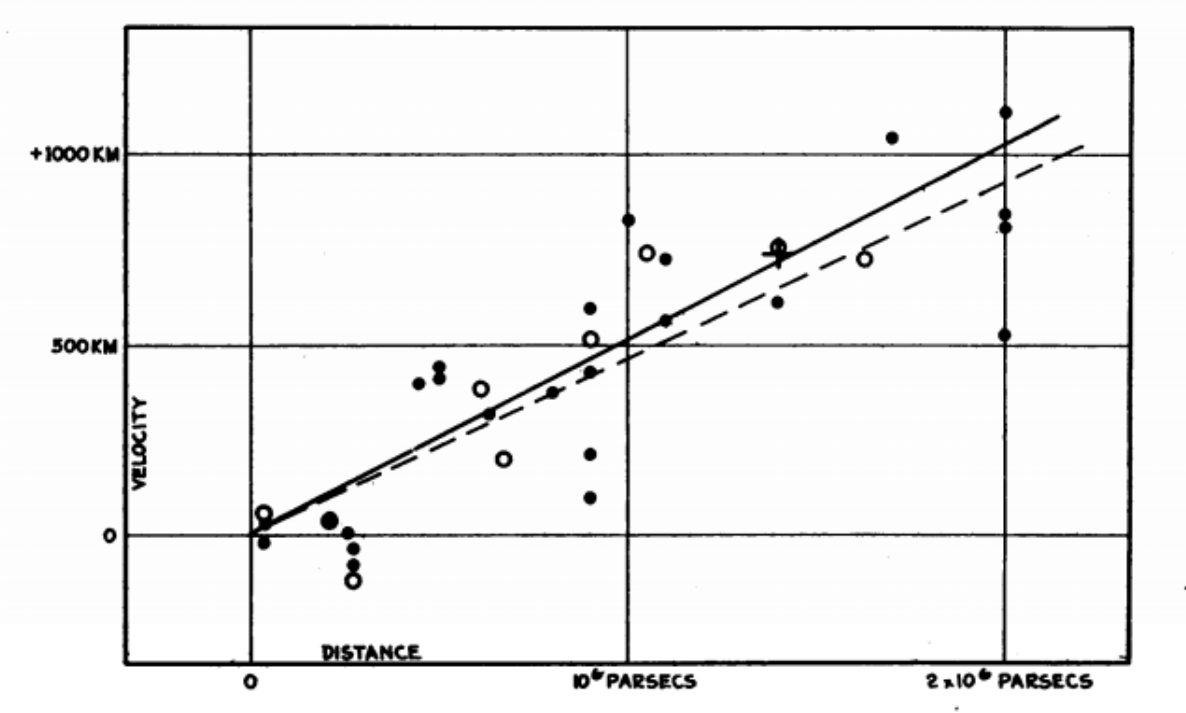
\includegraphics[width=0.8\textwidth]{MainLayout/Introduction_chapter/figures/hubble_og.png}
    \caption{Original Hubble diagram (\cite{Hubble_1929}) portraying the distance velocity diagram of nearby galaxies.}
    \label{fig:hubble_og}
\end{figure}

\subsection{Friedmann-Lemaitre-Robertson-Walker Metric}

We present here a metric that satisfies the homogeneity and isotropy of the Universe as well as an expanding one called Friedmann-Lemaître-Robertson-Walker (FLRW). It is more convenient 
to express the metric in spherical coordinates $(t, r, \phi, \theta)$. Working in natural units $c=1$, we obtain:
\begin{equation}
    ds^2 = dt^2 - a^2(t)\left[ \frac{dr^2}{1-kr^2} + r^2(d\theta^2 + \sin^2(\theta)d\phi^2) \right]
\end{equation}
where $a(t)$ is a dimensionless parameter called the "scale" factor, defined such that today at $t_0$ it is equal to 1, and used to describe the expansion which can be written as :

\begin{equation}
    H(t) = \frac{\dot{a}(t)}{a(t)}
\end{equation}
where the dot denotes the derivative with respect to time and $H(t)$ the Hubble parameter. 
$k$ is a global curvature term such that it can take one of three values $0,-1,1$ to describe a Universe that is flat, open/hyperbolic or closed/spherical respectively.
It is important to note that we can obtain the redshift of an object that emitted a wave at a time $t_e$ from the scale factor as the following relation holds true:
\begin{equation}
    \frac{a(t_0)}{a(t_e)} = 1+z
\end{equation}
Often we apply a change of coordinates such that any object maintains its coordinates regardless of the expansion. These are called comoving coordinates. We define the 
comoving distance $\chi$ such that:
\begin{equation}
    r = S_k(\chi) = \begin{cases}
        S_0(\chi) = \chi \\
        S_{1}(\chi) = \sin(\chi) \\
        S_{-1}(\chi) = \sinh(\chi)
    \end{cases}
\end{equation}
\begin{equation}
    d\chi = \frac{dr}{\sqrt{1-kr^2}}
\end{equation}

The metric then becomes : 
\begin{equation}
    ds^2 = dt^2 - a^2(t)\left[ d\chi^2 + S_k^2(\chi) (d\theta^2 + \sin^2(\theta)d\phi^2) \right]
\end{equation}

\subsection{Friedmann Equations}

Since the Universe is assumed to be homogeneous and isotropic, we can express the energy-momentum tensor $T^{\mu \nu}$ only as a time-dependent object describing the density $\rho$ and pressure 
$P$ of all components present in the Universe. We assume that these can be described as a perfect fluid with no viscosity. For each fluid present indexed by $i$, we can then write down the pressure 
term as $P_i=w_i\rho_i c^2$ where $w$ is the equation of state parameter. This gives us the following form for $T^{\mu \nu}$:
\begin{equation}
    T^{\mu \nu}_i = \rho_i \left[ (w_i+1)u^{\mu}u^{\nu} + w_ig^{\mu \nu} \right]
    \label{eqn:T_mu_nu}
\end{equation}
with $u^{\mu}$ being the velocity vector of the fluid. The local conservation of energy and momentum is expressed by $\nabla_{\mu} T^{\mu \nu} =0 $ where $\nabla_{\mu}$ is the covariant derivative. \\

Using this, the Einstein equations and the FLRW metric, Friedmann derived the following equations known as the Friedmann equations in 1924 (\cite{Friedmann_1922, Friedmann_1924}): 

\begin{equation}
    H^2 = \left( \frac{\dot{a}}{a} \right)^2 = \sum_i \frac{8 \pi G}{3}\rho_i - \frac{kc^2}{a^2}
    \label{eqn:friedmann_1}
\end{equation}
\begin{equation}
    \frac{\ddot{a}}{a} = - \sum_i\frac{4\pi G}{3}\left(\rho_i + 3 \frac{P_i}{c^2}\right)
    \label{eqn:friedmann_2}
\end{equation}

The first equation describes how fast the Universe is expanding knowing the Universe's composition $\rho_i$ and curvature $k$, while the second describes its acceleration.
Combining equations \ref{eqn:friedmann_1} and \ref{eqn:friedmann_2} we get:

\begin{equation}
    \frac{\dot{\rho_i}}{\rho_i} = -3(w_i+1)\frac{\dot{a}}{a}
\end{equation}

And the solution to this differential equation is:

\begin{equation}
    \boxed{\rho_i(t) = \rho_i(t_0)a(t)^{-3(w_i+1)}}
\end{equation}

This entails that the evolution of the scale factor is entirely determined by the nature of the fluids present at a time $t$. Knowing $w$ of each fluid informs us on the behaviour of 
$a(t)$. If we consider one fluid that dominates, the scale factor can be written as:
\begin{equation}
    a(t) \sim t^{\frac{2}{3(1+w)}}
\end{equation}

Consequently, the value of $w$ of the dominant fluid determines the behaviour of the expansion:
\begin{equation}
    \begin{array}{lll}
    \ddot{a}>0 & w<-1/3 & \text{accelerated expansion} \\
    \ddot{a}=0 & w=-1/3 & \text{constant expansion} \\
    \ddot{a}<0 & w>-1/3 & \text{decelerated expansion}
    \end{array}
    \end{equation}

\subsection{Energy Contents of the Universe}

Within the current cosmological framework, the total energy density of the Universe is commonly divided into the following main components:
\begin{itemize}
    \item \textbf{Radiation} ($w_r = \frac{1}{3}$): a relativistic component composed primarily of photons and neutrinos. Its contribution is negligible in the present-day Universe, 
    but it dominated the energy budget during the earliest cosmological epochs.

    \item \textbf{Matter} ($w_m = 0$): a non-relativistic component including both baryonic matter and dark matter. While baryonic matter constitutes the visible content of galaxies, 
    the dominant fraction is dark matter, whose existence was first inferred from galaxy cluster dynamics by Zwicky (\cite{zwicky1933}, \cite{andernach2017}). In the standard cosmological model, dark matter is assumed to be cold, meaning that its particles were non-relativistic during the epoch of structure formation.

    \item \textbf{Cosmological constant / Dark energy} ($w_{\Lambda} = -1$): in the standard $\Lambda$CDM model, cosmic acceleration is described by the cosmological constant $\Lambda$, 
    interpreted as an intrinsic property of spacetime with equation of state $w=-1$. More generally, dark energy may be viewed as an additional fluid component 
    driving accelerated expansion. Possible deviations from $\Lambda$CDM include models with a constant but free equation of state ($w$CDM), or a time-evolving 
    equation of state such as the CPL parametrization (\cite{Chevallier_2001}).
\end{itemize}
\textcolor{red}{COMMENT : might be woth mentioning the quantum vacuum fluctuations and the order of magnitude issue}

The equations of state for matter and radiation can be determined using a statistical physics framework. 
For simplicity, we will not be going into the details of the derivations for each component but simply give the end 
results. \\
\noindent For non-relativistic species, such as matter, we obtain :
\begin{equation}
    w_m = 0
\end{equation}
\noindent For relativistic species, such as radiation, we obtain :
\begin{equation}
    w_r = \frac{1}{3}
\end{equation}

\noindent For the cosmological constant this can be determined without going through the statistical physics. 
Instead, it follows directly from General Relativity by interpreting the cosmological constant as an effective perfect fluid. 
Einstein's field equations can be written as:

\begin{equation}
    G_{\mu\nu}
    =
    \frac{8\pi G}{c^4}
    \left(
    T_{\mu\nu}
    +
    T_{\mu\nu}^{(\Lambda)}
    \right),
\end{equation}
where
\begin{equation}
    T_{\mu\nu}^{(\Lambda)}
    =
    -\frac{\Lambda c^4}{8\pi G}g_{\mu\nu}.
\end{equation}

\noindent Comparing this expression with the stress-energy tensor of a perfect fluid at rest-frame (Equation \ref{eqn:T_mu_nu} where $u^{\mu} = (c,0,0,0)$) 
shows that the cosmological constant behaves as a fluid with energy density:
\begin{equation}
    \rho_{\Lambda}
    =
    \frac{\Lambda c^2}{8\pi G},
\end{equation}
\noindent which is constant by construction since $\Lambda$ is assumed to be constant. Following the energy-momentum conservation we get:
\begin{equation}
    \dot{\rho}
    +
    3H\left(\rho+\frac{P}{c^2}\right)
    =
    0,
\end{equation}
\noindent which then implies:
\begin{equation}
    P_{\Lambda}
    =
    -\rho_{\Lambda}c^2,
\end{equation}
\noindent from which $w_{\Lambda}$ immediately follows,
\begin{equation}
    w_{\Lambda}
    =
    \frac{P_{\Lambda}}{\rho_{\Lambda}c^2}
    =
    -1.
\end{equation}

We introduce the critical density $\rho_c$ defined as the energy density of the Universe for $k=0$ and at $t=t_0$:
\begin{equation}
    \rho_{c,0} = \frac{3H_0^2}{8\pi G}
\end{equation}
This critical density is used to normalize the densities of the other fluids such that the normalized density is written as:
\begin{equation}
    \Omega_{i,0} = \frac{\rho_i(t_0)}{\rho_c}
\end{equation}
At $t=t_0$, the Friedmann equation yields $\Omega_{m,0} + \Omega_{r,0} + \Omega_{\Lambda,0} + \Omega_{k,0} = 1$ with $\Omega_{k,0}$ being the contribution from the curvature by construction at $t=t_0$:
\begin{equation}
    \Omega_{k,t_0} = \frac{-kc^2}{a(t_0)^2H_0^2}
\end{equation}
Equation \ref{eqn:friedmann_1} can be then rewritten as :
\begin{eqnarray}
    H(t) = H_0 \sqrt{ \Omega_{m,0} a(t)^{-3} + \Omega_{r,0} a(t)^{-4} +\Omega_{\Lambda,0} +\Omega_{k,0} a(t)^{-2}}
\end{eqnarray}


Current cosmological observations indicate that the present-day Universe is remarkably close to spatial flatness, corresponding to $\Omega_{k,0}\simeq 0$ 
\cite{Planck_2018_params}. The dominant contribution to the total energy budget is consistent with a cosmological constant (or dark energy), representing 
approximately $70\%$ of the total density. Matter contributes roughly $30\%$, of which about $25\%$ corresponds to dark matter and only $\sim5\%$ to baryonic matter. 
The radiation component today is subdominant, contributing less than $1\%$ of the total energy density. \\

The relative importance of these components evolves with cosmic expansion according to their different scalings with the scale factor. The evolution of 
each energy component is represented in Figure \ref{fig:omega_vs_a}. Since radiation 
scales as $a^{-4}$, matter as $a^{-3}$, and the cosmological constant remains constant, the early Universe was initially radiation dominated. As the Universe 
expanded and cooled, a transition to matter domination occurred, enabling the growth of gravitational instabilities and the formation of large-scale structure. 
At late times, the cosmological constant became dominant, driving the current phase of accelerated expansion. \\

\begin{figure}[ht]
    \centering
    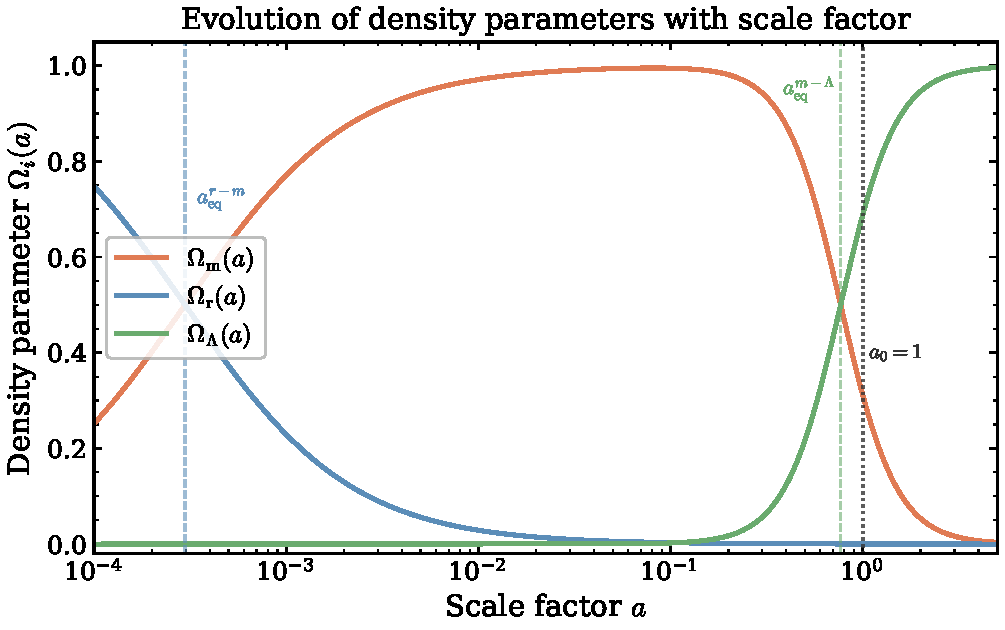
\includegraphics[width=1.0\textwidth]{MainLayout/Introduction_chapter/figures/omega_vs_a.pdf}
    \caption{Evolution of the main components of the $\Lambda$CDM model with respect to the scale factor. This highlights where each component dominates as well as when they become equal.}
    \label{fig:omega_vs_a}
\end{figure}


The acceleration of the Universe was confirmed by \cite{Riess_1998} and \cite{Perlmutter_1999} when they constructed a Hubble diagram with distant Type Ia supernovae. 
Each paper has shown that the supernova Hubble diagram cannot be solely explained with a Universe containing only matter and that an additional energy component must 
be accounted for. This is seen in Figure \ref{fig:hubble_riess}.\\


\begin{figure}[ht]
    \centering
    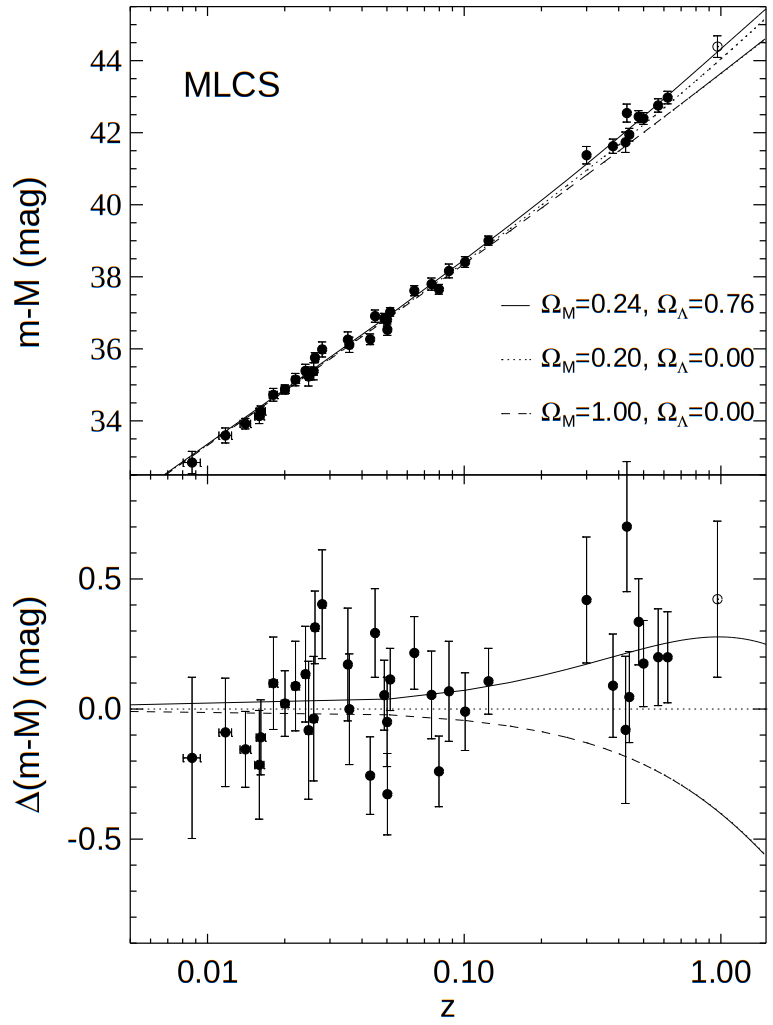
\includegraphics[width=0.7\textwidth]{MainLayout/Introduction_chapter/figures/hubble_riess_.png}
    \caption{Hubble diagram constructed using 50 Type Ia supernovae from \cite{Riess_1998} 
    along the predictions from three Universe models containing: only matter (20\% of the energy content) as a dotted line; 
    only matter (100\% of the energy content) as a dashed line; and matter (24\%) + $\Lambda$ (76\%) as a solid line. The data fits the solid line best.}
    \label{fig:hubble_riess}
\end{figure}

\subsection{The $\Lambda$CDM Model}

The $\Lambda$CDM model is the standard model of cosmology. It is built upon the framework of GR and assumes that the Universe began in an 
extremely hot and dense state, known as the Hot Big Bang, and has been expanding ever since. As the Universe expanded and cooled, it underwent three 
successive epochs of domination by different energy components, each governing the dynamics of expansion through the Friedmann equations: a radiation 
dominated era at early times, followed by a matter dominated era, and finally the current dark energy dominated era driven by the cosmological 
constant $\Lambda$. \\

The energy content of the Universe in $\Lambda$CDM consists of the components introduced in the previous section: radiation, baryonic matter, cold dark matter 
and a cosmological constant $\Lambda$, with their present-day fractions measured to be approximately $\Omega_r \approx 9 \times 10^{-5}$, $\Omega_b \approx 0.05$, 
$\Omega_{\text{CDM}} \approx 0.26$ and $\Omega_\Lambda \approx 0.69$ respectively 
(\cite{Planck_2018_params}), in a spatially flat Universe where $\sum_i \Omega_i = 1$. The model makes the additional assumptions that the 
Universe is homogeneous and isotropic on large scales (the cosmological principle), and that the primordial density perturbations seeding all structures are adiabatic 
and nearly Gaussian (\cite{Planck_2018}). \\

The $\Lambda$CDM model is fully characterised by six independent cosmological 
parameters:

\begin{itemize}
    \item $A_s$ — the amplitude of primordial scalar perturbations
    \item $n_s$ — the spectral index of the primordial power spectrum
    \item $\Omega_b h^2$ — the physical baryon density
    \item $\Omega_{\text{CDM}} h^2$ — the physical cold dark matter density
    \item $\theta_*$ — angular size of the sound horizon at recombination 
    \item $\tau$ — the optical depth to reionization
\end{itemize}

All other cosmological quantities, such as $\Omega_\Lambda$, $\sigma_8$ and $S_8$, are derived from these six parameters within the model. 
For example, $\sigma_8$ can be related to $A_s$ such that:
\begin{equation}
    \sigma_8 \propto \sqrt{A_s}
\end{equation}
Despite its simplicity, $\Lambda$CDM has proven remarkably successful in describing a wide range of observations, from the CMB anisotropies (\cite{Planck_2018_params}) to the 
large-scale distribution of galaxies (\cite{DESI_DR2_2025}), the BAO standard ruler 
(\cite{Eisenstein_2005}), and the accelerated expansion of the Universe (\cite{Riess_1998, Perlmutter_1999}). Nevertheless, as discussed in Section 
\ref{sec:tensions}, emerging tensions between different observational probes suggest that $\Lambda$CDM may require extensions or modifications.\\

The $\Lambda$CDM model is founded on the Hot Big Bang paradigm, whose success rests on three major observational pillars. These pillars are:
\begin{itemize}
    \item Expansion of the Universe as observed by Hubble in \cite{Hubble_1929}.
    \item Big Bang Nucleosynthesis (BBN) which predicts the primordial abundances of light elements (hydrogen, helium, and lithium) formed at the very early stages of the Universe (\cite{Cyburt_2016}, \cite{Wagoner_1967}).
    \item Cosmic Microwave Background (CMB), the trace of thermal radiation released when the Universe cooled sufficiently for protons 
    and electrons to recombine into neutral hydrogen at $z \sim 1100$ (\cite{Penzias_1965_a}, \cite{Penzias_1965_b}) (more details in Section \ref{section:cmb}). 
\end{itemize}
Together, these three pillars provide strong evidence for a hot, dense early Universe that has been expanding and cooling ever since. \\


Although $\Lambda$CDM describes the Universe as homogeneous and isotropic at the largest scales, this description breaks down at smaller scales where 
structures such as galaxies and galaxy clusters emerge. Explaining the emergence of inhomogeneous structures from an initially homogeneous Universe, while preserving the 
assumptions of $\Lambda$CDM, is an important challenge. We describe this process in the following section. \\